\documentclass[twoside]{article}
\setlength{\oddsidemargin}{0.25 in}
\setlength{\evensidemargin}{-0.25 in}
\setlength{\topmargin}{-0.6 in}
\setlength{\textwidth}{6.5 in}
\setlength{\textheight}{8.5 in}
\setlength{\headsep}{0.75 in}
\setlength{\parindent}{0 in}
\setlength{\parskip}{0.1 in}

\usepackage{graphicx}
\usepackage{url}

%
% The following commands sets up the lecnum (lecture number)
% counter and make various numbering schemes work relative
% to the lecture number.
%
\newcounter{lecnum}
\renewcommand{\thepage}{\thelecnum-\arabic{page}}
\renewcommand{\thesection}{\thelecnum.\arabic{section}}
\renewcommand{\theequation}{\thelecnum.\arabic{equation}}
\renewcommand{\thefigure}{\thelecnum.\arabic{figure}}
\renewcommand{\thetable}{\thelecnum.\arabic{table}}
\newcommand{\dnl}{\mbox{}\par}

%
% The following macro is used to generate the header.
%
\newcommand{\lecture}[4]{
  \pagestyle{myheadings}
  \thispagestyle{plain}
  \newpage
  \setcounter{lecnum}{#1}
  \setcounter{page}{1}
  \noindent
  \begin{center}
  \framebox{
     \vbox{\vspace{2mm}
   \hbox to 6.28in { {\bf CMPSCI~590S~~~Systems for Data Science
                       \hfill Fall 2017} }
      \vspace{4mm}
      \hbox to 6.28in { {\Large \hfill Lecture #2  \hfill} }
%       \hbox to 6.28in { {\Large \hfill Lecture #1: #2  \hfill} }
      \vspace{2mm}
      \hbox to 6.28in { {\it Lecturer: #3 \hfill Scribe: #4} }
     \vspace{2mm}}
  }
  \end{center}
  \markboth{Lecture #1: #2}{Lecture #1: #2}
  \vspace*{4mm}
}


\renewcommand{\cite}[1]{[#1]}

% \input{epsf}

%Use this command for a figure; it puts a figure in wherever you want it.
%usage: \fig{NUMBER}{FIGURE-SIZE}{CAPTION}{FILENAME}
\newcommand{\fig}[4]{
           \vspace{0.2 in}
           \setlength{\epsfxsize}{#2}
           \centerline{\epsfbox{#4}}
           \begin{center}
           Figure \thelecnum.#1:~#3
           \end{center}
   }

% Use these for theorems, lemmas, proofs, etc.
\newtheorem{theorem}{Theorem}[lecnum]
\newtheorem{lemma}[theorem]{Lemma}
\newtheorem{proposition}[theorem]{Proposition}
\newtheorem{claim}[theorem]{Claim}
\newtheorem{corollary}[theorem]{Corollary}
\newtheorem{definition}[theorem]{Definition}
\newenvironment{proof}{{\bf Proof:}}{\hfill\rule{2mm}{2mm}}

% Some useful equation alignment commands, borrowed from TeX
\makeatletter
\def\eqalign#1{\,\vcenter{\openup\jot\m@th
 \ialign{\strut\hfil$\displaystyle{##}$&$\displaystyle{{}##}$\hfil
     \crcr#1\crcr}}\,}
\def\eqalignno#1{\displ@y \tabskip\@centering
 \halign to\displaywidth{\hfil$\displaystyle{##}$\tabskip\z@skip
   &$\displaystyle{{}##}$\hfil\tabskip\@centering
   &\llap{$##$}\tabskip\z@skip\crcr
   #1\crcr}}
\def\leqalignno#1{\displ@y \tabskip\@centering
 \halign to\displaywidth{\hfil$\displaystyle{##}$\tabskip\z@skip
   &$\displaystyle{{}##}$\hfil\tabskip\@centering
   &\kern-\displaywidth\rlap{$##$}\tabskip\displaywidth\crcr
   #1\crcr}}
\makeatother

% **** IF YOU WANT TO DEFINE ADDITIONAL MACROS FOR YOURSELF, PUT THEM HERE:



% Some general latex examples and examples making use of the
% macros follow.

\begin{document}

%FILL IN THE RIGHT INFO.
%\lecture{**LECTURE-NUMBER**}{**DATE**}{**LECTURER**}{**SCRIBE**}
\lecture{2}{September 7}{Emery Berger}{Aishwarya Kamath, Ananya Suraj}

\section{General Memory Model}

Memory can be thought of as a big array. For example, in a 64 bit architecture, the size of a word is 8 bytes. The memory array would have to be of size $2^61 \approx 10^19 \approx 2$ billion gigabytes!
Hence, this general memory model which looks like the one in Figure \ref{fig:gmm}, is unrealistic. 

\begin{figure}[htp]
	\centering
  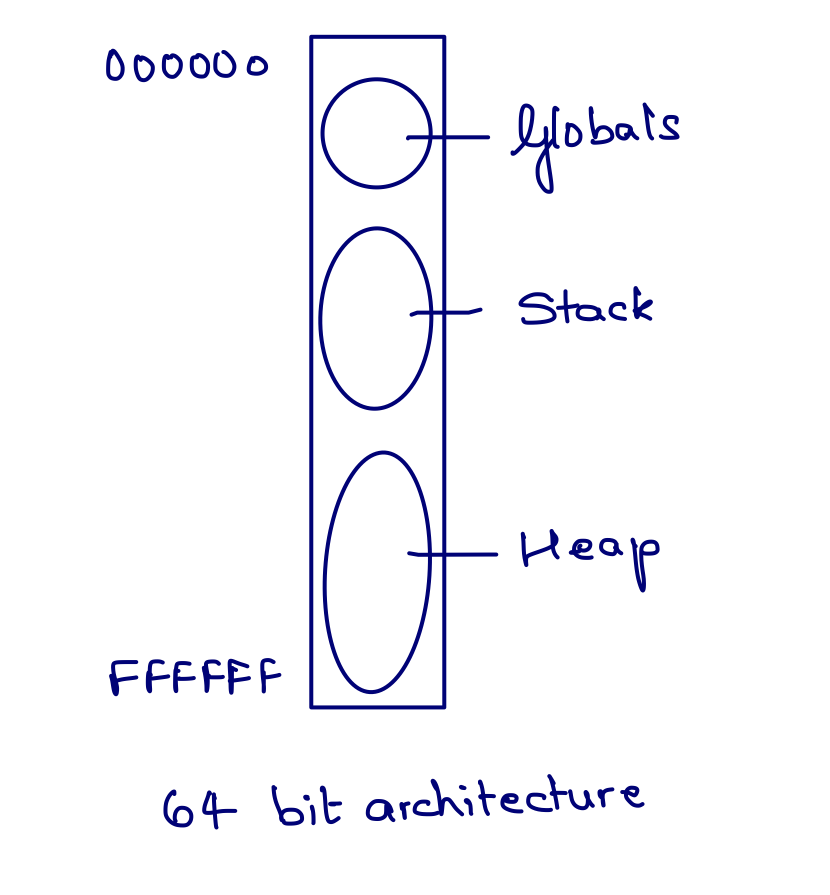
\includegraphics[width=0.2\linewidth]{Image-1.png}
  \caption{General memory model}
  \label{fig:gmm}
\end{figure}

Limitations of using Physical Memory:
\begin{itemize}
\item Portability: If physical memory addresses are used, transferring objects from one machine to another becomes impossible as the physical address that is used to refer to the object will change on the new machine.
\item Isolation: If two or more users are running programs at the same time and use physical addresses, a memory error in one program (for example, reading a bad pointer) could destroy memory being used by the other process, taking down multiple programs due to a single crash.
\item Limited Memory: Since physical memory addresses would just be from say, 00000000 to FFFFFFFF, this puts a big limitation on the user as one generally needs a lot more memory in practice. Virtual Memory which is a solution to these limitations is discussed in the next section.
\end{itemize}

\subsection{Virtual memory}
We use an abstraction called "Virtual Memory" which was invented in the 1960s. The operating system still sees the physical memory but the user sees the virtual memory layer. The idea behind virtual memory is the following : "All problems are solved by adding one level of indirection". 

Consider a user who looks for an item at address 1,000,000. This is the item's address in virtual memory which is a "view" of the data actually stored in physical memory. The mapping to the physical memory is called "translation" (Fig \ref{fig:translation}. The key idea here is to never give two objects the same memory. So, if another user tries to access the same variable, suppose, it gets mapped to a different chunk of physical memory. Locations in physical memory are completely separate though the virtual address may appear to be the same. 

\begin{figure}[htp]
	\centering
  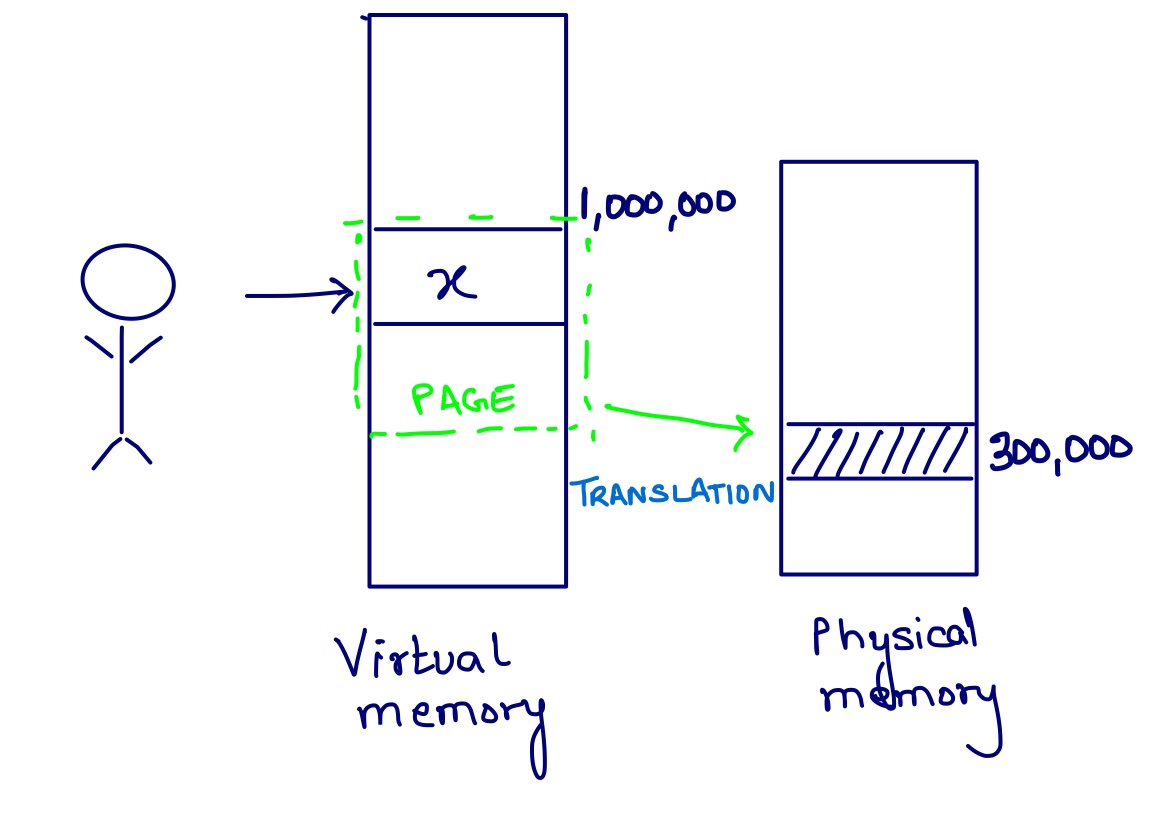
\includegraphics[width=0.4\linewidth]{Image-1.jpg}
  \caption{Translation}
  \label{fig:translation}
\end{figure}


The issue that arises now is, what happens when RAM gets filled?\\ \\
\textbf {Swapping} is the technique used to combat this problem. Pages that are rarely used are swapped out of memory to bring in new pages from the disk. A separate part of disk called the "swap partition" is assigned the task of holding swapped out data. By default, 4-8 times the size of RAM is saved on the disk for swap on Macs. Linux systems use a separate logical disk as a swap partition Fig \ref{fig:swap}.

\begin{figure}[htp]
	\centering
  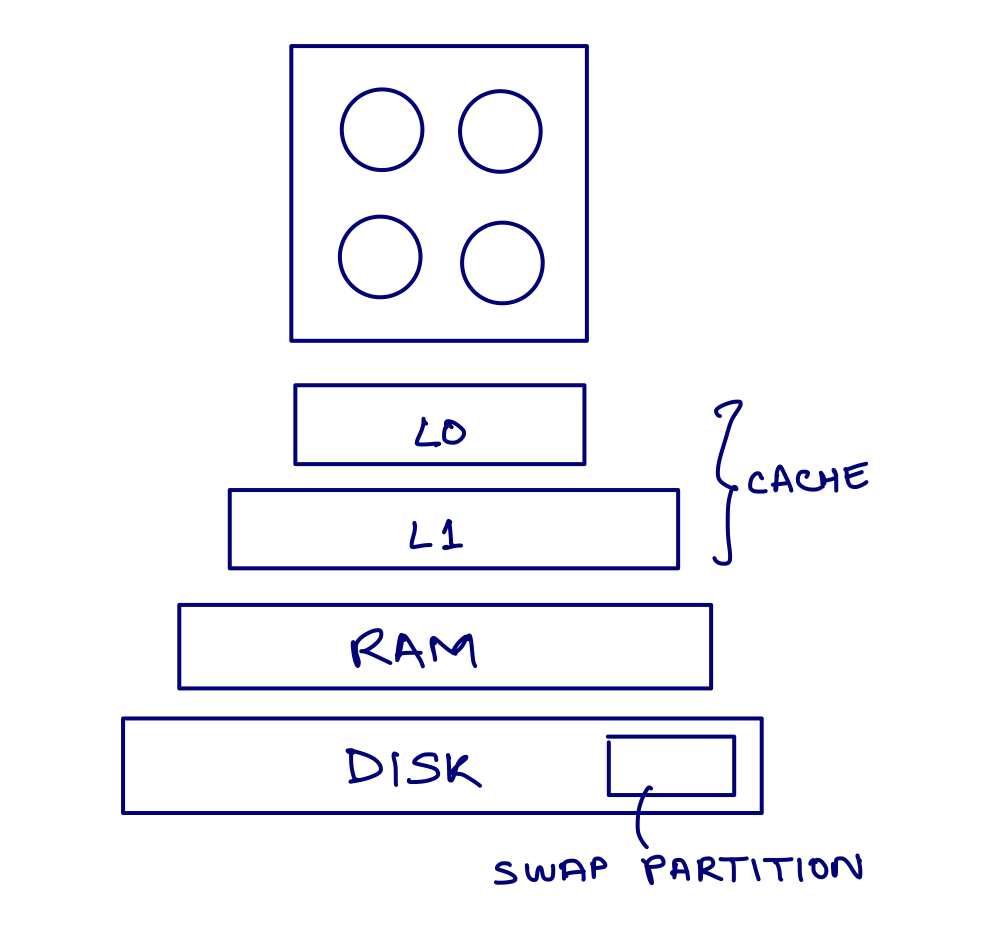
\includegraphics[width=0.4\linewidth]{Image-1-1.png}
  \caption{Swap partition}
  \label{fig:swap}
\end{figure}


A method of virtual memory management called demand paging is used, in which the pages of data are not copied from disk to RAM until they are needed. This is in contrast to anticipatory paging, also called page pre-fetch, in which pages that will be referenced soon as predicted and fetched, so as to reduce the future page faults. 
\\
\subsection{Strategies for Eviction}
Eviction is the term used to describe taking pages out from cache and putting it on disk. 
\begin{itemize}
\item \textbf {Least Recently Used (LRU)} : This cache replacement policy replaces the least recently used page from the cache with the latest page that was accessed. In order to implement this kind of caching mechanism, the state of every page will have to be maintained. One way to do this would be to have a counter for the time stamp at which a page was last accessed and increment it every time the page is accessed again. At the time of eviction, the page with the earliest time stamp is thrown out. An example of LRU strategy is the Clock Page Replacement algorithm.
\item \textbf {Random} : This strategy does not require to keep track of the state. 
Surprisingly, both these strategies do equally badly. For the random strategy, the odds of getting unlucky - that we would require to fetch data that is on disk and not in memory - is very small. In the case of LRU, it can go from 100\% hit to 0\% hit in successive fetches as seen in Figure \ref{fig:lru}.   
\end{itemize}

\begin{figure}[htp]
	\centering
  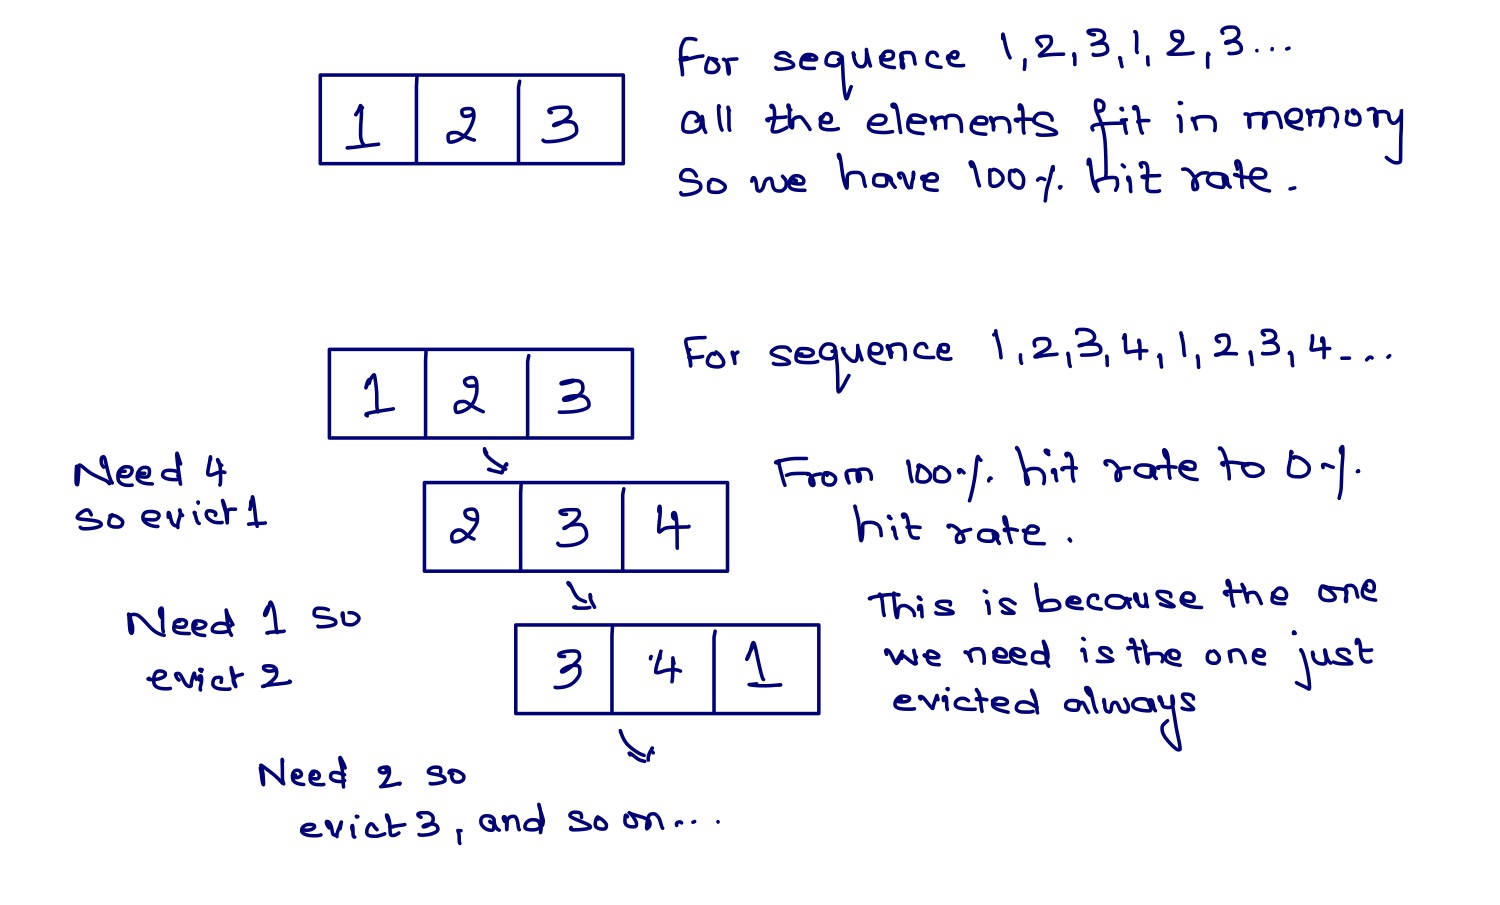
\includegraphics[width=0.5\linewidth]{Image-1-1.jpg}
  \caption{Least Recently Used Eviction}
  \label{fig:lru}
\end{figure}

\section{Use of Cache in Web Browsers}
In a web browser like Chrome, information is cached extensively so that websites can be accessed faster and data can be loaded quickly (Fig \ref{fig:www}). When a website gets a lot of hits, cache service companies like Akamai, Cloudflare etc help the websites by providing them with the required memory.    \\\\

\begin{figure}[htp]
	\centering
  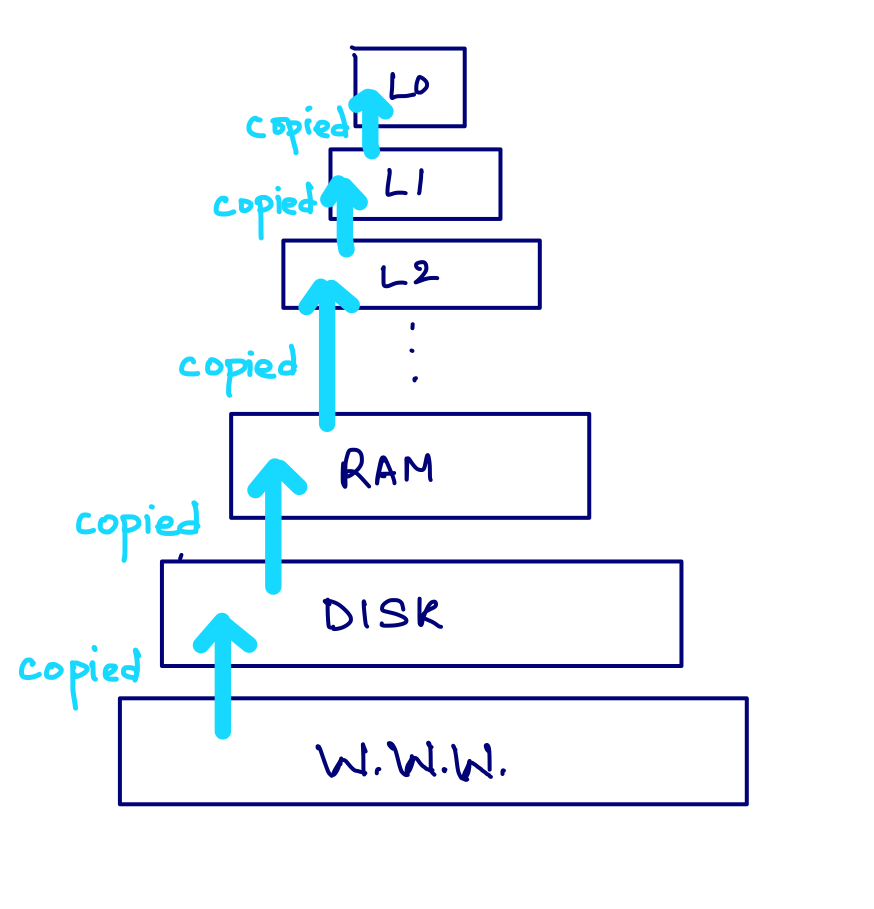
\includegraphics[width=0.3\linewidth]{Image-1-2.png}
  \caption{Web browser caching}
  \label{fig:www}
\end{figure}


\section{Translation Lookaside Buffer}

\textbf {A translation lookaside buffer(TLB)}, also known as an address translation cache, is a memory cache that reduces the time required to access a memory location. The Memory Management Unit (MMU) of a computer has the TLB which contains a few virtual to physical address mappings. The size of the TLB, in terms of number of entries is usually small from about 256 to 512 entries. The entries stored in the TLB are the virtual memory to physical memory translations of recently accessed memory locations (Fig \ref{fig:TLB}).

\begin{figure}[htp]
	\centering
  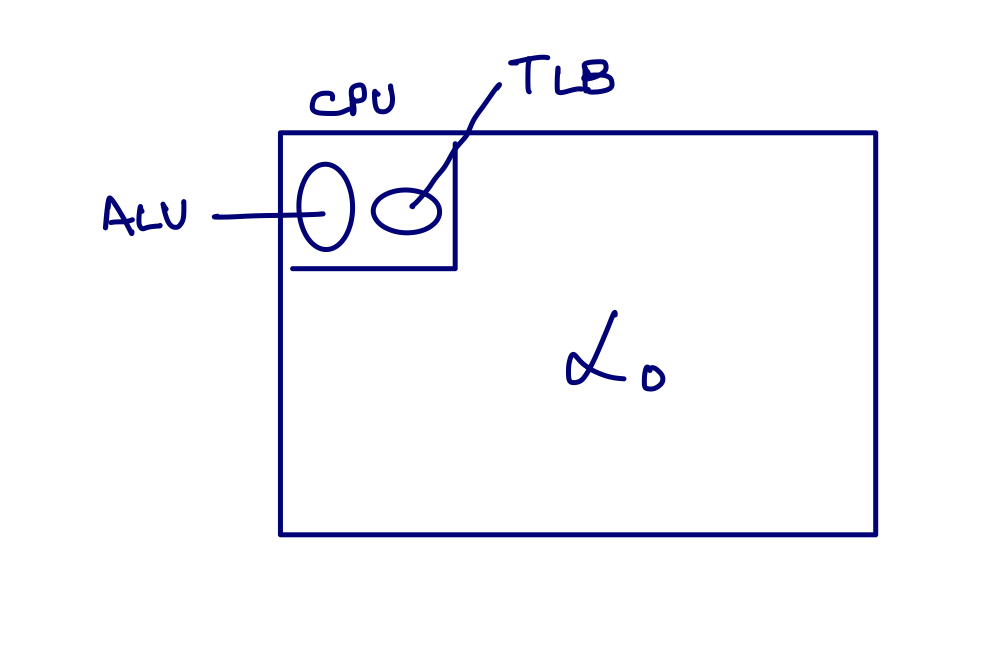
\includegraphics[width=0.3\linewidth]{Image-1-3.png}
  \caption{Translation Lookaside Buffer}
  \label{fig:TLB}
\end{figure}

The data structure used to store a TLB is not a hash table because hash functions do not maintain locality of the data. Trees are used instead so that the RAM stores sequential data in contiguous locations.

\textbf{High TLB Pressure}: 
Suppose the working set T has 512 entries in the TLB and the page size is around 4K, then we can only access 512 x 4K $\approx$ 2MB, which seems very insufficient as today even a small image has a size of about 3MB. Hence, having a very small page size puts a large amount of pressure on the TLB. 

\textbf{Solution}:
Dynamic Page Sizing: Some architectures support multiple page sizes with pages that can be significantly larger than the standard size (4K, 2MB or even 1GB). Operating systems like Linux support dynamic page sizes called Huge Pages, while Windows offers Large Pages and FreeBSD supports SuperPages. This reduces the pressure on the TLB. For example, if you often use 1GB of space, then it promotes the page size dynamically to 1GB.


\end{document}
